\section{Evaluation}

\subsection{Benchmarking}

In order to evaluate the performance of SFQ($D^2$) and compare it with
other schedulers, we implemented SFQ(D) and set up a benchmark
environment in a single cluster node, which has two six-core 2.4GHz Xeon CPUs
and 24GB of RAM, and a 120G MLC STAT SSD.
All experiments were conducted using FIO with direct IO directly
to the drive (i.e. no filesystem).

The first step was to benchmark the SSD to determine the optimal
device latency and the expected depth parameter. To do this, we
executed an FIO experiment of size 10GB, starting with the ``iodpeth''
parameter set to 1 and incrementing after each experiment. All
experiments are using random workloads. Figure~\ref{fig:latMot} shows
that latency grows more-or-less linearly as IO depth
increases. Figure~\ref{fig:bandMot} however, indicates that as IO
depth grows, bandwidth approaches some maximum value. Thus, it follows
that in order to maximize device throughput while maintaining a
reasonable per request latency, the optimal IO depth should be the
lowest possible depth that still achieves near maximum
bandwidth. Based on the data collected, we decided the optimal depth
would be somewhere between 11 and 13 for reads and 3 to 5 for
writes. This correlates with an average latency of 400 to 500
microseconds for reads and 100 and 190 microseconds to writes.

\begin{figure}[t]
  \centering 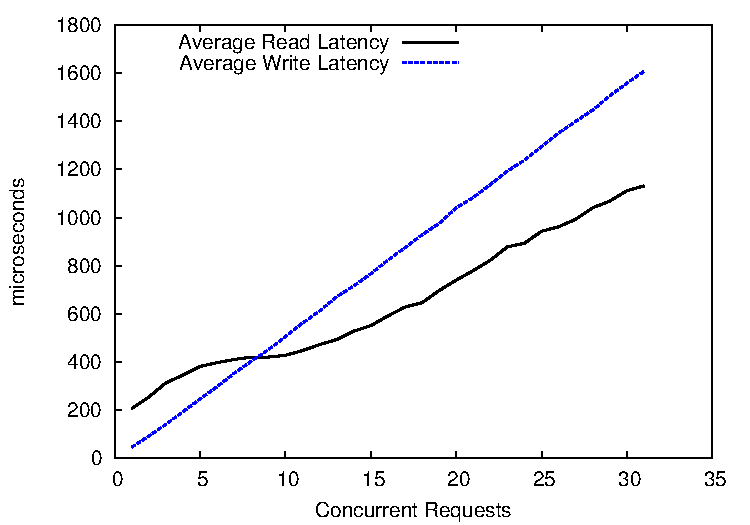
\includegraphics[width=\linewidth]{../../graphs/noop/latency_motivation.pdf}
  \caption{Average Latency vs IO depth}
  \label{fig:latMot}
\end{figure} 

\begin{figure}[t]
  \centering 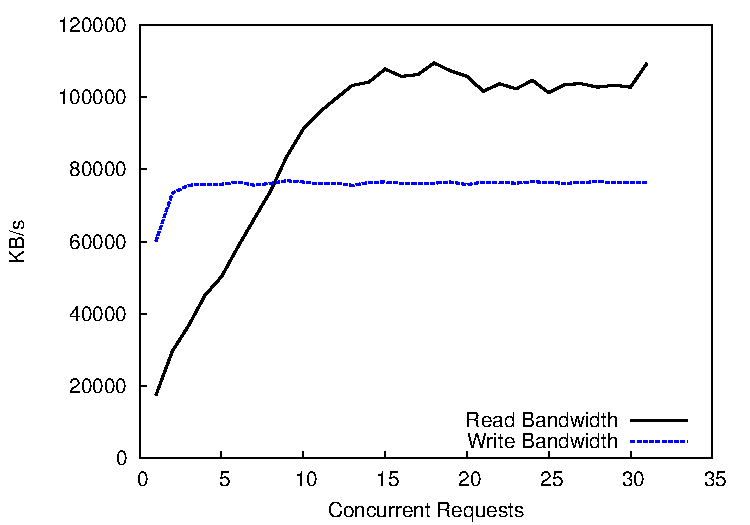
\includegraphics[width=\linewidth]{../../graphs/noop/bandwidth_motivation.pdf}
  \caption{Bandwidth vs IO depth}
  \label{fig:bandMot}
\end{figure}

\subsection{Isolated Workloads}

\begin{figure}[t]
  \centering 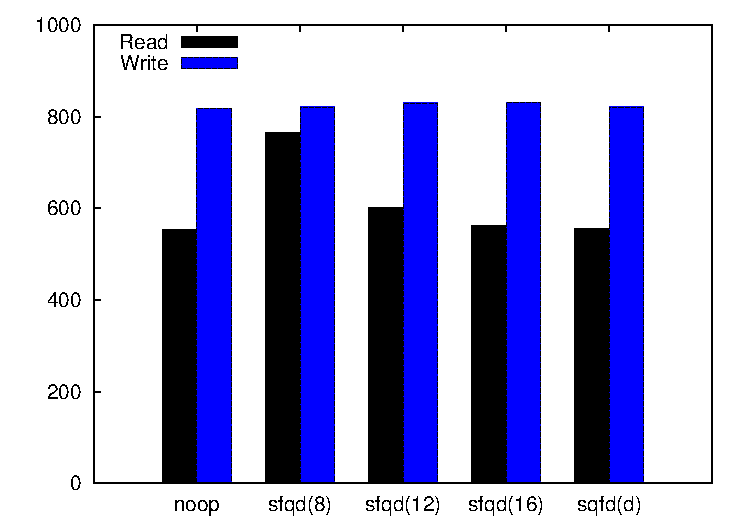
\includegraphics[width=\linewidth]{../../graphs/solo/latency.pdf}
  \caption{Average Latency for Isolated Workloads}
  \label{fig:latSolo}
\end{figure} 

\begin{figure}[t]
  \centering 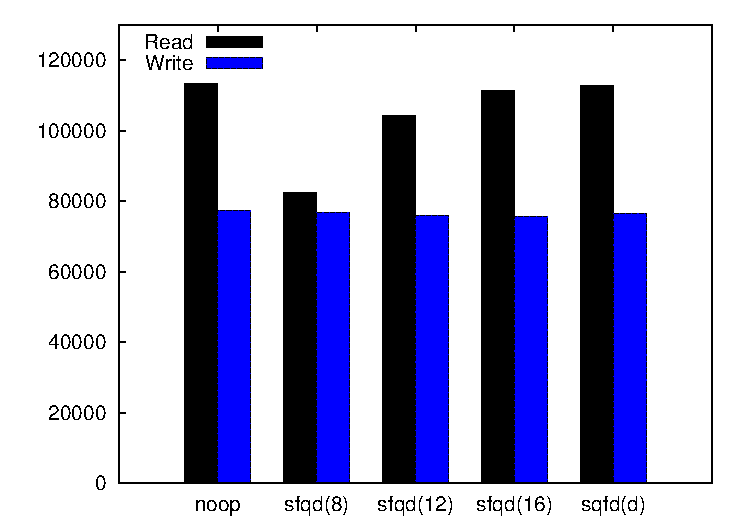
\includegraphics[width=\linewidth]{../../graphs/solo/bandwidth.pdf}
  \caption{Bandwidth for Isolated Workloads}
  \label{fig:bandSolo}
\end{figure}

To verify implementation, we first compared our implementations using
random read and write workloads. Figure~\ref{fig:latSolo} and
figure~\ref{fig:bandSolo} depict the latency and bandwidth results,
respectively. The x-axis represents which scheduler was used: noop,
SFQ(D) with depth 8, 12 and 16, and SFQ($D^2$). SFQ($D^2$)'s target
latency values are set to 100 and 481 microseconds for reads and
writes respectively.

We believe that noop represents the optimal throughput, and, in fact,
it does report the best results of all implementations. The statistics
reported are collected by FIO, so latency is application level, not
what is observed by the scheduler. As you can see SFQ(D) with D=16 and
SFQ($D^2$)'s performances match that of NOOP. In this experiment, we
observed that SFQ($D^2$)'s I/O depth converged with the optimal IO
depth explained in the previous subsection. At the very least, we see
that SFQ($D^2$) exhibits close to optimal bandwidth and does not
introduce significant overhead to IO performance.

\section{Competive Workloads}

In order to quanitify SFQ($D^2$)'s ability to schedule multiple
processes fairly we evaluated each scheduler with two concurrent
instances of FIO. One workload is a heavy streaming writter and the
other is a sparse sychronous reader. This experiment encompasses the
use case highlighted in the FlashFQ paper; we expect the reader will
forfeit its timeslice while it ``thinks'' between synchronous IOs and
suffer significant performance degridation in SFQ(D). 

\begin{figure}[t]
  \centering 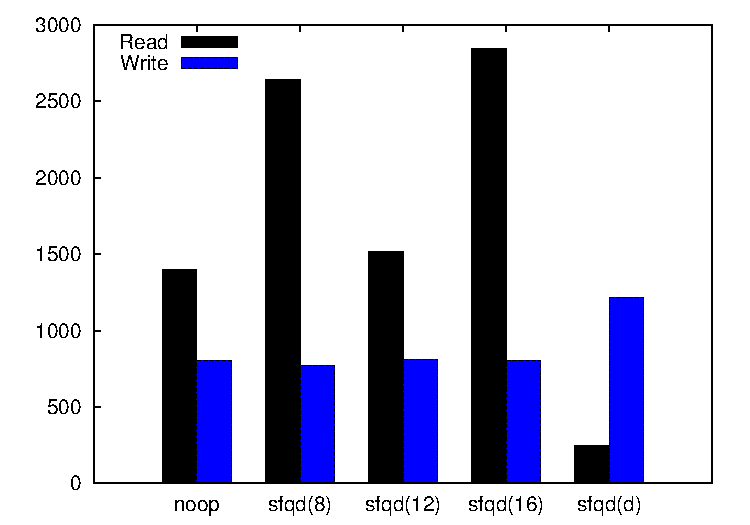
\includegraphics[width=\linewidth]{../../graphs/against/latency_against.pdf}
  \caption{Average Latency for Competitive Workloads}
  \label{fig:latAgs}
\end{figure} 

\begin{figure}[t]
  \centering 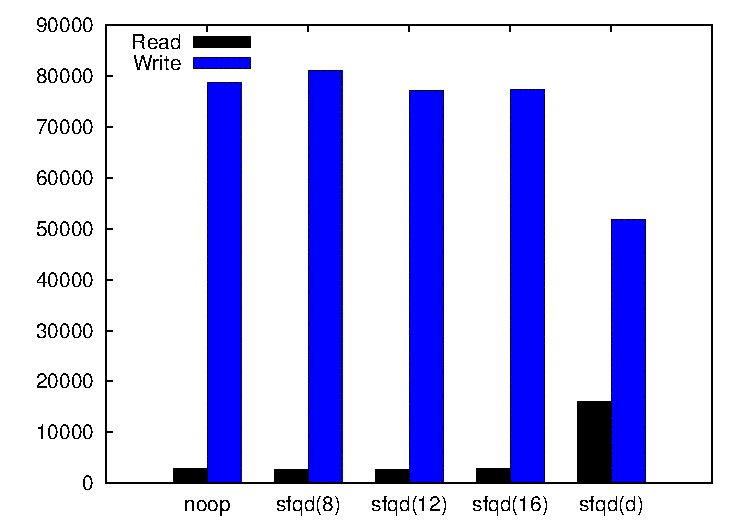
\includegraphics[width=\linewidth]{../../graphs/against/bandwidth_against.pdf}
  \caption{Bandwidth for Competitive Workloads}
  \label{fig:bandAgs}
\end{figure}

Figures~\ref{fig:latAgs} and~\ref{fig:bandAgs} show the results of
these experiments. As you can see, from figure~\ref{fig:latAgs}, the
read requests suffer much from high latency. This is due to device
saturation. The write latency is more-or-less stable until we get to
SFQ($D^2$), where it takes a slight hit, but comes with a massive
improvement for the read workload. Perhaps more interesting are the
bandwidth numbers. SFQ($D^2$) sees a sharp improvement in the read
throughput while writes, again take a hit. 

The increase in read bandwidth comes from the fact that the device
remains unsaturated from reduced IO depth enforced by
SFQ($D^2$). Thus, latencies are much lower than if the device had been
saturated so requests wait for much less time once they reach the
front of their process queue. The read requests are promoted within
the scheduler since they never use all of their timeslices and don't
have to wait as long a write request to finish before being
dispatched. 
